\documentclass[a4paper]{scrreprt}

% Uncomment to optimize for double-sided printing.
% \KOMAoptions{twoside}

% Set binding correction manually, if known.
% \KOMAoptions{BCOR=2cm}

% Localization options
\usepackage[english]{babel}
\usepackage[T1]{fontenc}
\usepackage[utf8]{inputenc}

% Sub figures
\usepackage{subcaption}

% Quotations
\usepackage{dirtytalk}

% Floats
\usepackage{float}

% Enhanced verbatim sections. We're mainly interested in
% \verbatiminput though.
\usepackage{verbatim}

% Automatically remove leading whitespace in lstlisting
\usepackage{lstautogobble}

% CSV to tables
\usepackage{csvsimple}

% PDF-compatible landscape mode.
% Makes PDF viewers show the page rotated by 90°.
\usepackage{pdflscape}

% Advanced tables
\usepackage{array}
\usepackage{tabularx}
\usepackage{longtable}

% Fancy tablerules
\usepackage{booktabs}

% Graphics
\usepackage{graphicx}

% Current time
\usepackage[useregional=numeric]{datetime2}

% Float barriers.
% Automatically add a FloatBarrier to each \section
\usepackage[section]{placeins}

% Custom header and footer
\usepackage{fancyhdr}

\usepackage{geometry}
\usepackage{layout}

% Math tools
\usepackage{mathtools}
% Math symbols
\usepackage{amsmath,amsfonts,amssymb}
\usepackage{amsthm}
% General symbols
\usepackage{stmaryrd}

% Utilities for quotations
\usepackage{csquotes}

% Bibliography
\usepackage[
  style=alphabetic,
  backend=biber, % Default backend, just listed for completness
  sorting=ynt % Sort by year, name, title
]{biblatex}
\addbibresource{references.bib}

\DeclarePairedDelimiter\abs{\lvert}{\rvert}
\DeclarePairedDelimiter\floor{\lfloor}{\rfloor}

\pagestyle{plain}

% Source code & highlighting
\usepackage{listings}

% SI units
\usepackage[binary-units=true]{siunitx}
\DeclareSIUnit\cycles{cycles}

% Should use this command wherever the print date is mentioned.
\newcommand{\printdate}{\today}

\newcommand{\mailsubject}{63112 Data Management Data Structures - Summary}
\newcommand{\maillink}[1]{\href{mailto:#1?subject=\mailsubject}
                               {#1}}

\subject{63112 Data Management Data Structures}
\title{Summary}

\author{Michael Senn \maillink{michael.senn@students.unibe.ch} --- 16-126-880}

\date{\printdate}

% Needs to be the last command in the preamble, for one reason or
% another. 
\usepackage{hyperref}

\begin{document}
\maketitle

\chapter{Introduction}

\begin{itemize}
		\item Different ways to classify data structures
				\begin{itemize}
						\item Probabilistic structures either trade off some
								incorrect queries for a more compact
								representation (e.g. bloom filter), or use
								randomness for data layout (e.g. skiplist)
						\item Persistent structures have built-in capabitlities
								to offload parts, or all of it, to storage
						\item Non-persistent ones assume they will live fully
								in memory
						\item Scalable
						\item Compressed
						\item Hash-based, Graph-Based, ...
				\end{itemize}
		\item Generic data structures able to store anything, as well as
				specific ones for e.g. text, grpah, geo data, ...
\end{itemize}

\chapter{B trees}

\section{Motivation}

\begin{itemize}
		\item Fast lookups over data which might not fit in memory
		\item Efficient insertion and deletion (compared to e.g. sorted array)
\end{itemize}

\section{Variations}

\begin{itemize}
		\item B* tree: Each node $\geq 2/3$ full
		\item B+ tree: Data only in leaf nodes
		\item B-link tree: Nodes on each level form linked list
		\item Often, tree with all these features also called B+ tree
\end{itemize}

\section{Layout}

\begin{itemize}
		\item Leaf nodes store data, either directly, or as pointer to actual
				resource
		\item Intermediary nodes contain separator keys which split data range
				of leaf nodes down their respective paths
		\item Large fanout factor (e.g. 100) means most space used for leaf
				nodes. Allows to e.g. cache all non-leaf nodes in memory even
				for gigantic tree.
\end{itemize}

\section{Operations}

\begin{itemize}
		\item Lookup traverses tree using separator keys until leaf node found
		\item Range lookups can then use leaf-level links to travel to next leaf
		\item On insertion, node might have to be split in two, with new separator key
		\item On deletion, nodes might have to be merged. Or we simply don't do this
\end{itemize}

\section{Buffer pool}

\begin{itemize}
		\item Allows retrieving pages by logical ID
		\item Allows retrieving fresh page
		\item Can be asked to pin/unpin/flush pages
		\item Handles associated disk IO if page not loaded
		\item Caches pages (LRU, random, ...) in memory
\end{itemize}

\subsection{Optimizations}

\begin{itemize}
		\item Pointer swizzling: Pointers to page IDs can, when page is loaded
				(and they point to a page which is /also/ loaded), be turned
				into direct pointers to memory
\end{itemize}

\section{Various}

\begin{itemize}
		\item Read (write) amplification: Actual amount of data read (written)
				compared to data we meant to read (write)
		\item B+-tree is read-oriented
		\item Unsuitable for variable keys (no stable fence keys) or large keys
				(not many keys per page)
\end{itemize}

\chapter{LSM trees}

\section{Motivation}

\begin{itemize}
		\item Write-oriented structure which still must support somewhat-efficient reads
		\item E.g. logging sensor metrics, or transaction logs
		\item In a B-tree a single 16B insert might cause 2-3 IOPS and 4KB of
				data written. Not ideal.
\end{itemize}

\section{Structure}

\textbf{Key insight} defer putting new data to persistent storage. Two
components: One memory-resident, one disk-resident.

\begin{itemize}
		\item $C_0$ tree: In-memory component (very freeing, needn't care about
				pages). Commonly done with e.g. Skiplist or AVL tree.
		\item Inserts done into $C_0$ tree (and logged, for resiliency)
		\item $C_0$ periodically compacted (merged) with on-disk $C_1$ component
		\item With inserts meanwhile going into new $C_0$ component
		\item $C_1$ can be done as fully loaded B-Tree. Or SSTables.
		\item SSTables: Shallow tree for variable-length keys.
\end{itemize}

\subsection{SSTable layout (example)}

\begin{itemize}
		\item Multi-level structure.
		\item Metadata of each SSTable: Key range (min, max), bloom filter,
				fixed-size index mapping key to approximate location in file.
		\item Fixed-size index can be achieved by e.g. using potentially
				shortened separator keys, or subset of actual keys.
		\item Lookup thus requires some traversal in structure
		\item Actual data is sorted values, e.g. key-value pairs sorted by key.
\end{itemize}

\section{Operations}

\begin{itemize}
		\item Insertion: Log (resiliency), the insert to $C_0$
		\item Compaction: Once $C_0$ full, flush to first disk tier. Write
				*new* SSTable.
		\item Merging: When $C_k$ full, merges entries of $C_k$ and produces
				non-overlapping SSTables for $C_{k+1}$ tier
		\item Lookup: Starting top down, for each SSTable: First check range.
				Then bloom filter. Then approximate location using fixed-size
				index. Then scan until data (or tombstone) found. Proceed to
				next level if not found.
		\item Deletion using tombstones
\end{itemize}

\chapter{Probabilistic structures}

\section{Motivation}

\begin{itemize}
		\item Use non-determinism for either a more compact representation (at
				the cost of inaccurate queries)
		\item Or for determining the topology of the data structure
		\item Index lookups can be expensive if they don't produce a hit. Goal:
				Structure in front which can cheaply catch large amount of
				these before they hit the index.
\end{itemize}

\section{Excerpt Hashing}

\begin{itemize}
		\item Numerical hashing (division): $h(x) = x \bmod m$, choice of $m$
				essential.  Primes not too close to power of two good.
		\item Numerical hashing (multiplication): $h(x) = \floor{m \cdot A}
				\bmod m$, choice of $m$ less important. $A$ can be e.g. golden
				ratio. But more expensive than division.
		\item String hashing: Use characters as coefficients of polynomial
				(rolling around).
		\item String hashing: Or FNV, MurmurHash3, very-fast hash functions
		\item All of these non-cryptographic, e.g. no collision resistance!
\end{itemize}

\section{Bloom filters}

\begin{itemize}
		\item Bitmap with $m$ bits
		\item $k$ hash functions which map to one of $m$ bits (just take
				regular hash functions $\bmod m$)
		\item To add element, hash with each function. Set bits which it maps to.
		\item To check, equivalently
		\item Can make hash functions use disjoint sets of bitmaps to prevent
				contention during bit access.
		\item More space for bitmap lowers false positiity rate. Or, keeping
				false positivity rate equal, allows using fewer hash functions
				(= faster).
		\item Issues: No resizing, no deletion, no data locality so must be
				in-memory for reasonable performance.
\end{itemize}

\section{Counting data structures}

\begin{itemize}
		\item Motivation: Keep track of unique visitors, or cardinality of a column
		\item Naive approach: Keep list of sorted values. But then $O(log n)$
				insertion and $O(n)$ space.
		\item Alternatives: Hashing will bring updates down to constant time,
				but still linear space. Sampling will trade off accuracy
				(especially for low-frequency values!) for lower space usage.
\end{itemize}

\subsection{Linear counting}

\begin{itemize}
		\item Bitmap with $m$ bits
		\item To insert, hash with one function and set corresponding bit
		\item With $z$ bits set, estimator of count is then $-m \cdot ln(1 - z/m)$
		\item Accuracy depends on load factor, so cardinality must be roughly known upfront
		\item Required space to keep error low is proportional to cardinality
\end{itemize}

\subsection{Probabilistic counting}

\begin{itemize}
		\item Instead of setting bit $h(x)$, set the bit corresponding to the rightmost $1$ in $h(x)$
		\item Then bits on left are way less likely to be set than bits on right (same idea as hash-based POW)
		\item Given leftmost $0$ at position $n$, estimator is then $2^n/0.77$
		\item But expected margin of error is 78 percent
		\item Can be offset by using several such counters. Use hash output to select which counter to update.
		\item Average of these counters can lower error margin to 10 percent for 64 maps.
\end{itemize}

\section{Probabilistic balanced trees}

\subsection{Background: Balanced trees}

\begin{itemize}
		\item Balance of node determined by difference in depth of right vs
				left subtree
		\item If difference exceeds 1, node is unbalanced
		\item Balanced binary trees enforce balance by means of left- and
				right-rotation around unbalanced nodes
		\item RB trees relax the requirement to allow easier implementation:
				Nodes are red or black, root is black, leaf nils are black, if
				node is red then both children are black.
		\item Then all paths from node to leaves have equal number of black
				trees
		\item Insertion is red
		\item RB guarantees at most two rotations are needed on
				insertion/deletion, though node must be able to change colour.
\end{itemize}

\subsection{PRNGs}

\begin{itemize}
		\item Sequence of pseudo-random numbers based on initial seed
		\item Empirical tests
				\begin{itemize}
						\item Frequency: Uniform distribution in $[0, 1]$
						\item Serial: Pairs of successive numbers must be
								uniformly distributed
						\item Gap: Gaps between occurrences of number $x$
						\item Run: Length of monotone parts of sequence
						\item Partition test, coupon collector's test, ...
				\end{itemize}
		\item LCG: Modulus $m > 0$, multiplier $0 < a < m$, increment $0 < c <
				m$, starting value $0 < x_0 < m$. Output: $x_{n+1} = (a x_n +
				c) \bmod m$.
		\item LCG is fast, but not uniform on hyperplane, and not secure at all
\end{itemize}

\subsection{Skiplist}

\begin{itemize}
		\item Represent tree as linked list
		\item Each node has $1$ to $n$ pointers to subsequent nodes
		\item Height $n$ of node randomly chosen
				\begin{itemize}
						\item If height was deterministically (e..g $k \mod n$
								for k-th node) then inserts would cause
								rebalancing of the whole remainder of the tree.
						\item With e.g. exponential falloff. Can be done as
								successive coin tosses.
				\end{itemize}
		\item Pointer at height $k$ points to next node with height $k$
		\item First and last node have maximum height $n$
		\item Lookup follows highest pointer until it would overshoot, then
				goes down one layer.
		\item Insertion does lookup, then insertion with randomized height
		\item Maximum height will not exceed $\log(n)$ in most cases
		\item Expected length of path is fraction of $\log(n)$
		\item Skiplists can be merged and concatenated in linear time
\end{itemize}

\chapter{Hashing}

\section{Addressing methods}

Recall: Hash function can be thought of as array, with values being hashed to
an address / offset within the array.

\begin{itemize}
		\item Closed addressing
				\begin{itemize}
						\item Elements kept at address they hash to
						\item In case of collisions, elements are chained
						\item If number of elements per bucket is high, resizing required
				\end{itemize}
		\item Open addressing
				\begin{itemize}
						\item In case of collision, probing method (linear,
								quadratic, ...) utilized to find place to put
								it
						\item Lookup stops when element, or empty slot, is
								found
						\item Worst-case insert and lookup performance $O(n)$,
								when having to traverse whole array
				\end{itemize}
\end{itemize}

\section{Universal hashing}

Hash function which is ideal for a given dataset, with as few collisions as
possible. Can sometimes be achieved by careful choice of hash function.

\section{Cuckoo addressing}

\begin{itemize}
		\item Idea: Split hash table in two, use two hash functions
		\item $h_1$ maps to first table, $h_2$ to second
		\item Item will be found in either first or second table
		\item Lookup and deletion simply check both
		\item Insertion of $x$: Will be stored at position $h_1(x)$
				\begin{itemize}
						\item If $h_1(x)$ already occupied by $y$, $y$ will be displaced to $h_2(y)$
						\item if $h_2(y)$ already occupied by $z$, $z$ will be displaced to $h_1(z)$
						\item ...
				\end{itemize}
		\item Cycles can occur during insertion and are tricky to detect, as
				only cycle if same slot visited twice with same originating
				element
				\begin{itemize}
						\item Storing whole trace is expensive. Heuristic: Maximum chain
								length, e.g. $\log_2(n)$ if $n$ slots
						\item On (probably) cycle: Resize table or change hash function
				\end{itemize}
		\item Insight: Few elements cause cycles. Idea: Use additional
				fixed-size stash where, if cycle detection kicks in, elements
				are kept
		\item Then during lookup, if cycle detected, stash is checked
\end{itemize}

\section{Hopscotch hashing}

\begin{itemize}
		\item Cuckoo's cache behaviour not ideal
		\item Insight: Make sure displaced location is near original location
		\item Single array, single hashfunction, hop-info bitmap of size $H$.
		\item Intuition: Item found at place it hashes to, or at most $H-1$
				positions after that.
		\item Insertion:
				\begin{itemize}
						\item If no collision, insert $x$ at $h(x)$ and set 0-th bit of bitmap
						\item If collision, displace existing (or new) item.
								Find empty slot within reach of bitmap, and set
								corresponding bit.
				\end{itemize}
		\item Reach of one field can contain fields occupied by displaced
				elements from other fields, do not touch those.
		\item If insertion finds no free space, do linear probing to find first
				unoccupied slot. Then, `bring free space closer' by moving
				items inbetween $h(x)$ and first free slot where their bitmaps
				permit, see figure \ref{img:hopscotch}.
		\item If we can't bring free space close enough, resize
		\item Capping $H$ to small value makes insertion, lookup, deletion $O(1)$
				\begin{itemize}
						\item Constants will be different, insertion might
								manipulate $k \cdot O(1)$ elements for some
								constant $k$.
				\end{itemize}
\end{itemize}

\begin{figure}
		\centering
		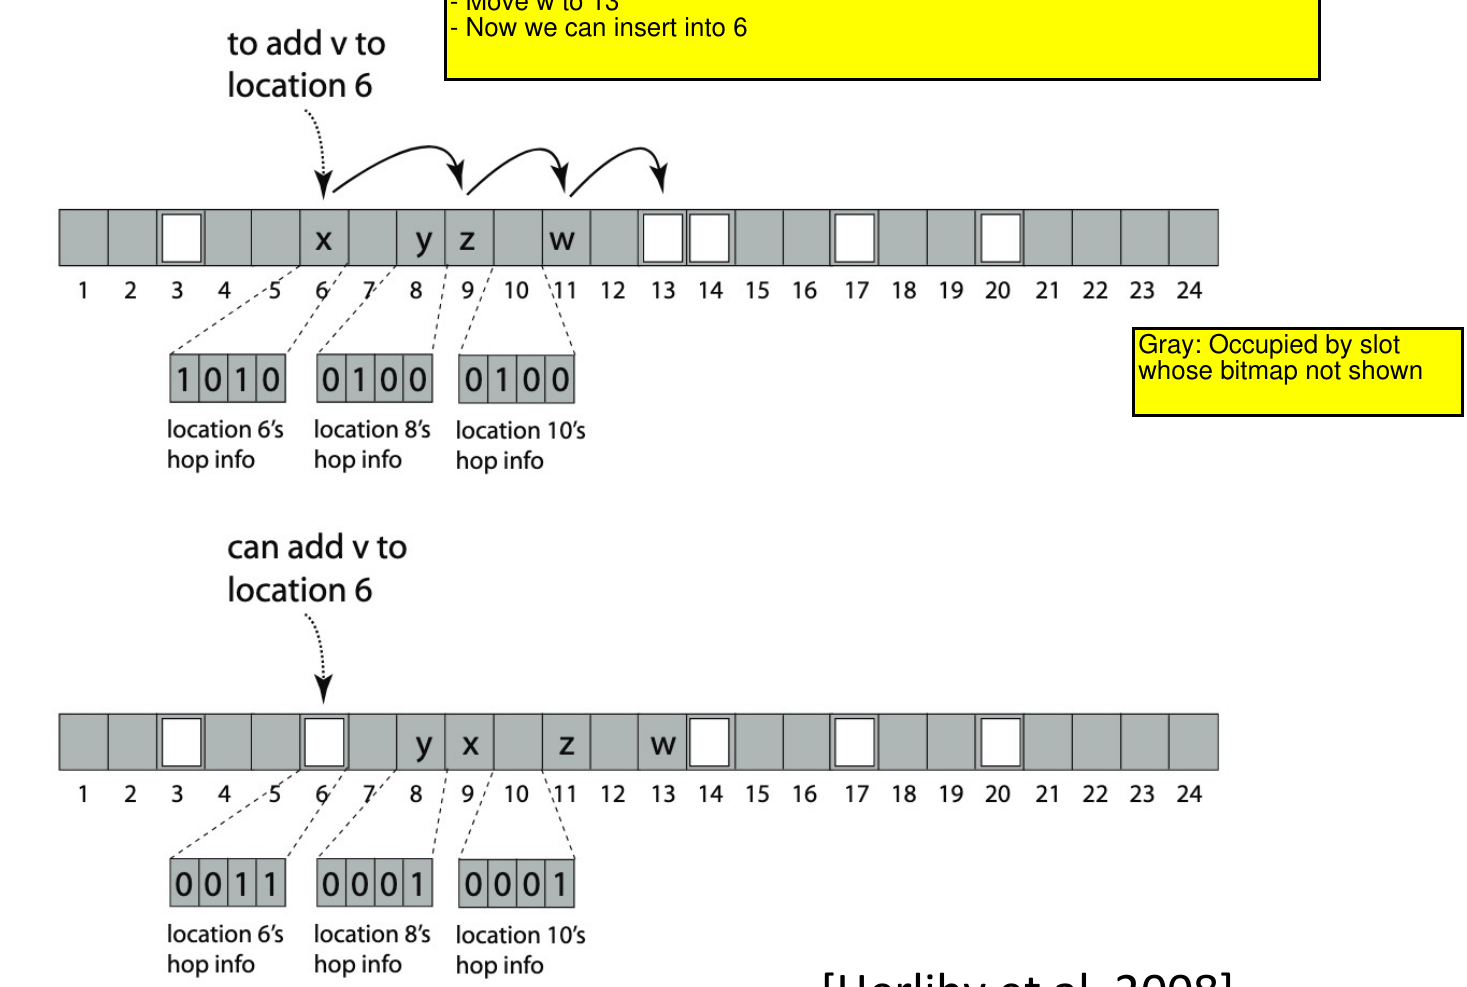
\includegraphics[width=\textwidth]{resources/07_hopscotch}
		\caption{Hopscotch hashing: Handling collisions \& lack of free space}
		\label{img:hopscotch}
\end{figure}

\section{Further improvements}

\begin{itemize}
		\item Swiss tables: SIMD instructions to test all keys in hop window at
				once
\end{itemize}

\chapter{LSM Recap, Tries, Various}

\begin{itemize}
		\item General idea: One region in memory, one in storage.
		\item Storage region has multiple tiers, growing (exponentially) in size
		\item Storage tiers often as skiplists
\end{itemize}

\section{Insertion}

\begin{itemize}
		\item Log for ACID purposes
		\item Insert in in-memory structure
\end{itemize}

\section{Compaction (flush memory to highest disk tier)}

\begin{itemize}
		\item Triggered once in-memory structure full
		\item Traverse memory structure, keep track of min/max
		\item Write new SSTable to first disk tier
\end{itemize}

\section{Merging (flush disk to lower disk tier)}

\begin{itemize}
		\item Triggered once disk tier $k$ full
		\item Merges upper-tier SSTables into lower-tier SSTables
		\item Creates non-overlapping SSTables (more performant for future lookups and merging)
		\item This causes write amplification
\end{itemize}

\section{SStable layout}

\begin{itemize}
		\item Immutable file
		\item Metadata
				\begin{itemize}
						\item Key range (min/max): Allows to check at a glance whether key might be contained within
						\item Bloom filter: Further prevent lookups of nonexistant keys
						\item Fixed-size index providing lookup of key to
								approximate location in SStable. Might use
								subset or trunated keys.
				\end{itemize}
		\item Data as sorted values (by key)
\end{itemize}

\subsection{Lookup}

\begin{itemize}
		\item Merge iterator
				\begin{itemize}
						\item Gathers all SSTables (based on min/max and bloom
								filter) which might contain key
						\item Gets initial position in file using approximate index
						\item Iterates over all remaining ones until it finds
								looked-up key, or iterator terminates
				\end{itemize}
\end{itemize}

\section{Column-oriented DBs}

\begin{itemize}
		\item When storing wide tuples, and wanting to e.g. aggregate along one dimension
		\item Define column families, which are columns often queried together
		\item Then store each primary key to family map in its own structure
\end{itemize}

\section{Indexing structures}

\begin{itemize}
		\item Hash based
		\item Trees
		\item Sorted arrays
		\item Tries
		\item Graphs
\end{itemize}

\section{Tries}

\begin{itemize}
		\item Prefix tree, keys spread along edges as e.g. bytes
		\item No balancing
		\item Lookup complexity depends on key length (opposed to B-tree, where logarithmic in number of keys)
		\item Lookup can terminate early (opposed to B-tree, where always to leaf)
\end{itemize}

\subsection{Representation}

\begin{itemize}
		\item Each node as fixed-size array of pointers
		\item E.g. fanout factor = 1 byte
		\item Looking up key then is a constant-time lookup in each node's array
		\item Span: Number of bits to represent part of key encoded in one
				node. E.g. span = 8 for byte fanout.
				\begin{itemize}
						\item Small span leads to compact representation with
								large depth, large span to sparse
								representation with shallow depth.
				\end{itemize}
		\item $count$ equal nodes with value $node$ can be compacted ot one
				$(count, node)$ meta-node.
\end{itemize}

\subsection{Example: Encoding DNA}

\begin{itemize}
		\item Fanout factor of four (ACTG)
		\item Per node:
				\begin{itemize}
						\item 4 pointers, 8B each
						\item 4 4B reference counters
						\item 4 1B bitmaps to mark whether pointers exist
								\begin{itemize}
										\item Alternatively use special value
												to indicate nonexistant
												pointer. Can be done as
												pointers are block-aligned, so
												invalid values exist.
								\end{itemize}
				\end{itemize}
		\item Insertion adds special terminator node to indicate existence of key
		\item And otherwise just sets pointers and increments counters along
				the way
		\item Deletion performs lookup to check key exists, then moves upwards
				to topmost node with reference counter (for appropriate edge)
				of 1, then deletes anything from there below.
		\item Reference counter could be per node, but then would need to dive
				down one more level to find out what to delete.
\end{itemize}

Heavily inefficient!

\printbibliography

\end{document}
